% This line sets the project root file.
% !TEX root = Notes_Gauging_Defects.tex
% !TEX spellcheck = en_US

\subsection{Fusion categories}

We briefly recall the definition of a fusion category, omitting many details. A full definition can be found in Chapter 4 of \cite{Etingof2015}.
\begin{definition}[Fusion category]
	A tensor category $\cat$ is a $\mathbb{C}$-linear category $\cat$ with a functor $\otimes:\cat\times\cat\to\cat$, a natural isomorphism $(-\otimes-)\otimes-\cong-\otimes(-\otimes-)$ called the associator, and a unit object $1$.
	These data must satisfy coherence equations such as the pentagon equations, that can be found in Sec. 2.1 of \cite{Etingof2015}.
	
	A \emph{fusion category} is a rigid \footnote{We refer the reader to \cite{Etingof2015} for details.} semisimple tensor category with finitely many isomorphism classes of simple objects and $\End(1)\cong \mathbb{C}$.
	
	It is convenient to describe a fusion category $\cat$ using \emph{skeletal data}. This approach is standard in the (physics) literature, and amounts to picking representatives for each isomorphism class of simple object. The full fusion category can be canonically reconstructed from the skeletal data \cite{BBJSkeletal}. A \emph{skeletal fusion category} consists of:
	\begin{itemize}
		\item A finite set of simple objects $L_\mathcal{C}=\{1,a,b,c,\ldots\}$ , where $1$ is the distinguished unit object.
		\item For each triple $(a,b;c)$ a finite dimensional Hilbert space $C(a\otimes b,c)$ represented as a trivalent vertex
		\begin{equation}
		\begin{tikzpicture}[scale=0.65,baseline=(current bounding box.center)]
		\draw (-.707,-.707)--(0,0) node[pos=-.25] {$a$};
		\draw (.707,-.707)--(0,0) node[pos=-.25] {$b$};
		\draw (0,0)--(0,1) node[pos=1.25] {$c$};
		\end{tikzpicture}.
		\end{equation} 
		\item An associator. If a basis is picked for each $C(-\otimes -,-)$ (here we assume these are all 1 dimensional for simplicity), the associator can be represented as a tensor $F$
		\begin{equation}
		\begin{tikzpicture}[scale=0.65,baseline=(current bounding box.center)]
		\draw (0,0)--(0,1) node[pos=1.25] {$d$};
		\draw (0,0)--(1.41,-1.41) node[pos=1.15] {$c$};
		\draw (0,0)--(-.707,-.707) node [pos=.5,above left] {$e$};
		\draw (-.707,-.707)--(-1.41,-1.41)node[pos=1.25] {$a$};
		\draw (-.707,-.707)--(0,-1.41)node[pos=1.25] {$b$};
		\end{tikzpicture}
		=\sum_{f\in L}\left(F_{abc}^{d}\right)_{e,f}
		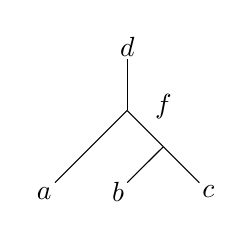
\begin{tikzpicture}[scale=0.65,baseline=(current bounding box.center)]
		\draw (0,0)--(0,1) node[pos=1.25] {$d$};
		\draw (.707,-.707)--(1.41,-1.41) node[pos=1.25] {$c$};
		\draw (0,0)--(.707,-.707) node [pos=.5,above right] {$f$};
		\draw (0,0)--(-1.41,-1.41)node[pos=1.15] {$a$};
		\draw (.707,-.707)--(0,-1.41)node[pos=1.25] {$b$};
		\end{tikzpicture}.\label{eqn:Fsymbdef}
		\end{equation} 
		The tensors are often called the $F$-symbols.
	\end{itemize}
\end{definition}

\begin{example}[$\Vec(G)$]\label{example:vecG}
	Let $G$ be a finite group. The category $\Vec(G)$ is the category of $G$-graded vector spaces. The skeletal description is very simple. The set of simples is $G$ as a set, with the group identity becoming the unit. The vector spaces are 0 dimensional except $C(g\otimes h, gh)$ which is 1 dimensional for all $g,h$. The $F$-symbols are $+1$ when the diagrams in \eqref{eqn:Fsymbdef} are nonzero.
\end{example}